\documentclass[c]{beamer}
\usepackage{org-preamble}
\usepackage[cpp_teaching]{slide-style}
\usetheme{default}
\newcommand{\inline}[1]{\mintinline[breaklines]{c++}{#1}}


\title{Surcharge d'opérateur}

\begin{document}

\maketitle

%-------------------------------

\begin{frame}[fragile]{Surcharge d'opérateur}

\begin{itemize}[<+->]
\item On voudrait pouvoir faire
\begin{minted}[fontsize=\footnotesize,samepage,mathescape,xrightmargin=0.5cm,xleftmargin=0.5cm]{c++}
Vecteur2D vec1 { .x=2, .y=3 };
Vecteur2D vec2 { .x=4, .y=5 };
vec1 += vec2;                          // addition de vec2 à vec1
Vecteur2D vec3 = (vec1 - vec2) * 0.7;  // différence puis mult. scalaire
...
\end{minted}

\item Fondamentalement, l'appel à un opérateur tel que \texttt{+}, \texttt{=}, \texttt{+=}, \texttt{++}, \texttt{<<}, \texttt{[]}, \texttt{()}, \texttt{!}\ldots{} est identique à l'appel d'une fonction/méthode

\item Par défaut, ces opérations ne sont pas définies sur les classes que l'on crée

\item Mais \structure{possibilité de (sur)définir} ces opérateurs comme n'importe quelle autre méthode
\end{itemize}

\end{frame}

%-------------------------------

\begin{frame}[fragile]{Exemple de surcharge de l'opérateur unaire \texttt{+=}}

\begin{onlyenv}<1>
\begin{minted}[fontsize=\footnotesize,samepage,mathescape,xrightmargin=0.5cm,xleftmargin=0.5cm]{c++}
// Déclaration
class Vecteur2D {
public:
  double x;
  double y;
};


\end{minted}
\end{onlyenv}
\begin{onlyenv}<2>
\begin{minted}[fontsize=\footnotesize,samepage,mathescape,xrightmargin=0.5cm,xleftmargin=0.5cm]{c++}
// Déclaration
class Vecteur2D {
public:
  double x;
  double y;

  void operator+= (const Vecteur2D& right);
};
\end{minted}
\end{onlyenv}
\pause
\vspace{1em}
\begin{minted}[fontsize=\footnotesize,samepage,mathescape,xrightmargin=0.5cm,xleftmargin=0.5cm]{c++}
// Définition
void Vecteur2D::operator+= (const Vecteur2D& right) {
  x += right.x;
  y += right.y;
}
\end{minted}
\end{frame}

%-------------------------------

\begin{frame}[fragile]{Exemple de surcharge de l'opérateur unaire \texttt{+=}}
\begin{minted}[fontsize=\footnotesize,samepage,mathescape,xrightmargin=0.5cm,xleftmargin=0.5cm]{c++}
// Définition
void Vecteur2D::operator+= (const Vecteur2D& right) {
  x += right.x;
  y += right.y;
}

// Utilisation
void main () {
  Vecteur2D vec1 {2, 3};
  Vecteur2D vec2 {4, 5};
  vec1 += vec2;
}
\end{minted}

\begin{cbox}
\begin{center}
\structure{\(\rightarrow\) équivalent à l'usage d'une méthode \texttt{ajoute} s'utilisant de la façon
 suivante \inline{vec1.ajoute(vec2);}}
\end{center}
\end{cbox}
\end{frame}

\begin{frame}[fragile]{Opérateurs unaires}
Pratique usuelle avec les opérations unaires : renvoyer le résultat de l'opération.\\

\begin{minted}[fontsize=\footnotesize,samepage,mathescape,xrightmargin=0.5cm,xleftmargin=0.5cm]{c++}
// Déclaration
class Vecteur2D {
  ...
  Vecteur2D& operator+= (const Vecteur2D& right);
};

// Définition
Vecteur2D& Vecteur2D::operator+= (const Vecteur2D& right) {
  x += right.x;
  y += right.y;
  return *this;
}
\end{minted}

\begin{cbox}
\begin{center}
\structure{\(\rightarrow\) utilisation du pointeur \texttt{this} qui retourne l'adresse de l'objet courant}
\end{center}
\end{cbox}

\end{frame}

%-------------------------------------------------------------------

\begin{comment}
\begin{frame}[fragile]{Surcharge de l'opérateur binaire \texttt{+} : Fonction amie}
Objectif :
\begin{minted}[fontsize=\footnotesize,samepage,mathescape,xrightmargin=0.5cm,xleftmargin=0.5cm]{c++}
Vecteur2D vec1 {2, 3};
Vecteur2D vec2 {4, 5};
Vecteur2D vec3 = vec1 + vec2;
\end{minted}
\pause
\vspace{1em}
Implémentation :
\begin{minted}[fontsize=\footnotesize,samepage,mathescape,xrightmargin=0.5cm,xleftmargin=0.5cm]{c++}
// Déclaration
class Vecteur2D {
  ...
  friend Vecteur2D operator+ (const Vecteur2D& left, const Vecteur2D& right);
};

// Définition
Vecteur2D operator+ (const Vecteur2D& left, const Vecteur2D& right) {
  return Vecteur2D(left.m_x + right.m_x, left.m_y + right.m_y);
}
\end{minted}
\end{frame}
\end{comment}

%----------------------------------------------

\begin{frame}[fragile]{Surcharge de l'opérateur binaire \texttt{+} : Méthode constante}
Objectif :
\begin{minted}[fontsize=\footnotesize,samepage,mathescape,xrightmargin=0.5cm,xleftmargin=0.5cm]{c++}
Vecteur2D vec1 {2, 3};
Vecteur2D vec2 {4, 5};
Vecteur2D vec3 = vec1 + vec2;
\end{minted}
\vspace{1em}
Implémentation :
\begin{minted}[fontsize=\footnotesize,samepage,mathescape,xrightmargin=0.5cm,xleftmargin=0.5cm]{c++}
// Déclaration
class Vecteur2D {
  ...
  Vecteur2D operator+ (const Vecteur2D& right) const;
};

// Définition
Vecteur2D Vecteur2D::operator+ (const Vecteur2D& right) const {
  return Vecteur2D {
    x + right.x,
    y + right.y
  };
}
\end{minted}
\end{frame}

%----------------------------------------------

\begin{frame}[fragile]{Surcharge de l'opérateur binaire \texttt{+} : Fonction globale}
Objectif :
\begin{minted}[fontsize=\footnotesize,samepage,mathescape,xrightmargin=0.5cm,xleftmargin=0.5cm]{c++}
Vecteur2D vec1 {2, 3};
Vecteur2D vec2 {4, 5};
Vecteur2D vec3 = vec1 + vec2;
\end{minted}
\vspace{1em}
Implémentation :
\begin{minted}[fontsize=\footnotesize,samepage,mathescape,xrightmargin=0.5cm,xleftmargin=0.5cm]{c++}
// Déclaration en dehors de la classe
Vecteur2D operator+ (const Vecteur2D& left, const Vecteur2D& right);

// Définition
Vecteur2D operator+ (const Vecteur2D& left, const Vecteur2D& right) {
  return Vecteur2D {
    left.x + right.x,
    left.y + right.y
  };
}
\end{minted}
\end{frame}

%--------------------------------------------------

\begin{frame}[fragile]{Accès d'un élément de matrice}
Imaginons une classe \inline{Matrice} qui stocke une matrice sous forme de tableau de \inline{double} linéaire :
\vspace{1em}
\begin{center}
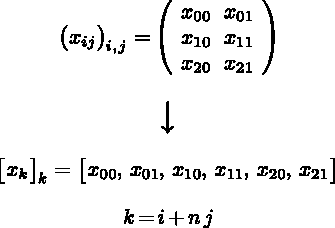
\includegraphics[width=0.4\paperwidth]{matrix-linear-storage.pdf}
\end{center}
\vspace{1em}
(cf. suite du cours) 
\end{frame}

\begin{frame}[fragile]{Accès d'un élément de matrice}

Une méthode \texttt{accès()} permet de récupérer l'élément $(\mathtt{row},\mathtt{col})$ :\\
\begin{minted}[fontsize=\footnotesize,samepage,mathescape,xrightmargin=0.5cm,xleftmargin=0.5cm]{c++}
class Matrice {
  double* data;
  unsigned int cols, rows;

public:
  ...
  double accès (int row, int col);  // Accès à un élément de la matrice
};

double Matrice::accès (int row, int col) {
  if (row < 0 or row >= rows or col < 0 or col >= cols)
    throw std::out_of_range();
  return data[ row*cols + col ];
}

cout << mat1.accès(1, 2) << endl;
\end{minted}

\end{frame}

\begin{frame}[fragile]{Accès d'un élément de matrice}

On peut la remplacer par un opérateur plus pratique :\\
\begin{minted}[fontsize=\footnotesize,samepage,mathescape,xrightmargin=0.5cm,xleftmargin=0.5cm]{c++}
class Matrice {
  double* data;
  unsigned int cols, rows;

public:
  ...
  double operator[] (int row, int col);  // Accès à un élément de la matrice
};

double Matrice::operator[] (int row, int col) {
  if (row < 0 or row >= rows or col < 0 or col >= cols)
    throw std::out_of_range();
  return data[ row*cols + col ];
}

cout << mat1[1,2] << endl;
\end{minted}

\end{frame}

%------------------------------------------------------------------

\begin{comment}
\begin{frame}[plain,label={sec:orgheadline12}]{}
\partpage
\end{frame}

\begin{frame}[label={sec:orgheadline13}]{Fonctions et classes amies}
\begin{itemize}
\item Du fait du principe d'encapsulation des données, les fonctions extérieures à
la classe n'ont pas accès aux membres privées de cette classe\ldots{}

\item \ldots{} à l'exception des fonctions amies

\item Utilité : quasi nulle sauf pour quelques opérations (dont la surcharge
d'opérateur)
\end{itemize}
\end{frame}

\begin{frame}[fragile,label={sec:orgheadline14}]{Exemple de fonction amie d'une classe}
 \begin{minted}[fontsize=\footnotesize,samepage,mathescape,xrightmargin=0.5cm,xleftmargin=0.5cm]{c++}
// Déclaration avec friend
class particule
{
  friend void stupid_thing(particule & particule_);
  ...
};
...
// Définition
void stupid_thing(particule & particule_)
{
  particule_.m_mass = 0.511;
}
...
// Utilisation
int main()
{
  particule muon(105.6, -1.6e-19);
  stupid_thing(muon);
}
\end{minted}
\end{frame}

\begin{frame}[fragile,label={sec:orgheadline15}]{Classe amie d'une autre classe}
 \begin{itemize}
\item Méthode d'une classe \texttt{B}, amie d'une autre classe \texttt{A}

\begin{minted}[fontsize=\footnotesize,samepage,mathescape,xrightmargin=0.5cm,xleftmargin=0.5cm]{c++}
class A
{
  ...
  friend void B::methode_de_B(A & A_);
  ...
};
\end{minted}

\item Classe \texttt{B} amie d'une autre classe \texttt{A}

\begin{minted}[fontsize=\footnotesize,samepage,mathescape,xrightmargin=0.5cm,xleftmargin=0.5cm]{c++}
class A
{
  ...
  friend class B;
  ...
};
\end{minted}
\end{itemize}
\end{frame}
\end{comment}

\end{document}
